%% fig_doublepoint.tex -- the local obstruction at an isolated double point.
%% Left: two smooth surfaces in a fourfold meeting transversally at a point
%% p, with their normal spaces N1, N2 at p, which together span T_p.
%% Centre: the bivectors at p, split as wedge^2 N1 + N1 (x) N2 + wedge^2 N2,
%% drawn as slabs of heights 1 : 4 : 1.  Right: the local Ext^2 of the germ
%% of the candidate at p in the two cases, the ideal I of the union and the
%% complex K of the separated branches, and which part of the bivectors the
%% products of the translation classes carry onto it.  The compensating
%% scalar has no germ at all, so the identity fails at points of both kinds.
\documentclass[tikz,border=9pt]{standalone}
\usepackage{amsmath,amssymb}
\usetikzlibrary{arrows.meta,calc,backgrounds,positioning,decorations.pathreplacing}
%% palette.tex -- shared colour definitions for the figures
\definecolor{PInk}{RGB}{26,32,44}
\definecolor{PBlue}{RGB}{37,82,139}
\definecolor{PTeal}{RGB}{23,127,125}
\definecolor{POchre}{RGB}{193,138,44}
\definecolor{PClay}{RGB}{178,74,58}
\definecolor{PSlate}{RGB}{108,122,137}
\definecolor{PViolet}{RGB}{110,86,150}
\definecolor{WBlue}{RGB}{223,234,246}
\definecolor{WTeal}{RGB}{220,238,236}
\definecolor{WOchre}{RGB}{250,240,218}
\definecolor{WClay}{RGB}{247,229,224}
\definecolor{WSlate}{RGB}{238,241,244}
\definecolor{PMag}{RGB}{158,58,110}
\definecolor{PGrass}{RGB}{62,124,66}
\definecolor{PAmber}{RGB}{214,112,38}
\definecolor{PIndigo}{RGB}{58,64,140}
\definecolor{PRule}{RGB}{176,186,197}

%% shared macros so the standalone figures match the paper
\providecommand{\QQ}{\mathbb{Q}}
\providecommand{\ZZ}{\mathbb{Z}}
\providecommand{\RR}{\mathbb{R}}
\providecommand{\CC}{\mathbb{C}}
\providecommand{\PP}{\mathbb{P}}
\providecommand{\Kx}{K^{\times}}
\providecommand{\HW}{W}
\providecommand{\Nm}{\mathrm{N}}
\providecommand{\Hdg}{\mathrm{Hdg}}
\providecommand{\NS}{\mathrm{NS}}
\providecommand{\cA}{\mathcal{A}}
\providecommand{\cD}{\mathcal{D}}
\providecommand{\cF}{\mathcal{F}}
\providecommand{\cP}{\mathcal{P}}
\providecommand{\cO}{\mathcal{O}}
\providecommand{\cQ}{\mathcal{Q}}
\providecommand{\bbar}[1]{\overline{#1}}
\providecommand{\ch}{\operatorname{ch}}
\providecommand{\End}{\mathrm{End}}


\tikzset{obl/.style={x={(1cm,0cm)}, y={(0.50cm,0.36cm)}, z={(0cm,1cm)}}}

\newcommand{\slab}[7]{%
  \begin{scope}[obl]
    \fill[#7 top]   (#1,#2,#3+#6) -- (#1+#4,#2,#3+#6) -- (#1+#4,#2+#5,#3+#6) -- (#1,#2+#5,#3+#6) -- cycle;
    \fill[#7 front] (#1,#2,#3) -- (#1+#4,#2,#3) -- (#1+#4,#2,#3+#6) -- (#1,#2,#3+#6) -- cycle;
    \fill[#7 side]  (#1+#4,#2,#3) -- (#1+#4,#2+#5,#3) -- (#1+#4,#2+#5,#3+#6) -- (#1+#4,#2,#3+#6) -- cycle;
    \draw[#7 edge]  (#1,#2,#3) -- (#1+#4,#2,#3) -- (#1+#4,#2,#3+#6) -- (#1,#2,#3+#6) -- cycle;
    \draw[#7 edge]  (#1+#4,#2,#3) -- (#1+#4,#2+#5,#3) -- (#1+#4,#2+#5,#3+#6) -- (#1+#4,#2,#3+#6);
    \draw[#7 edge]  (#1,#2,#3+#6) -- (#1,#2+#5,#3+#6) -- (#1+#4,#2+#5,#3+#6);
  \end{scope}}

\tikzset{
  zz top/.style={fill=WBlue},   zz front/.style={fill=WBlue!80!PBlue!30},
  zz side/.style={fill=WBlue!60!PBlue!40}, zz edge/.style={draw=PBlue,line width=0.55pt},
  vv top/.style={fill=WClay},   vv front/.style={fill=WClay!80!PClay!30},
  vv side/.style={fill=WClay!60!PClay!40}, vv edge/.style={draw=PClay,line width=0.55pt},
  pp top/.style={fill=PViolet!14!white}, pp front/.style={fill=PViolet!26!white},
  pp side/.style={fill=PViolet!36!white}, pp edge/.style={draw=PViolet,line width=0.55pt},
  ker top/.style={fill=WTeal},  ker front/.style={fill=WTeal!80!PTeal!35},
  ker side/.style={fill=WTeal!60!PTeal!45}, ker edge/.style={draw=PTeal,line width=0.9pt},
  sig top/.style={fill=WOchre}, sig front/.style={fill=WOchre!80!POchre!35},
  sig side/.style={fill=WOchre!60!POchre!45}, sig edge/.style={draw=POchre,line width=0.9pt},
  ext top/.style={fill=WSlate}, ext front/.style={fill=WSlate!85!PSlate!20},
  ext side/.style={fill=WSlate!70!PSlate!30}, ext edge/.style={draw=PSlate,line width=0.5pt},
}

\begin{document}
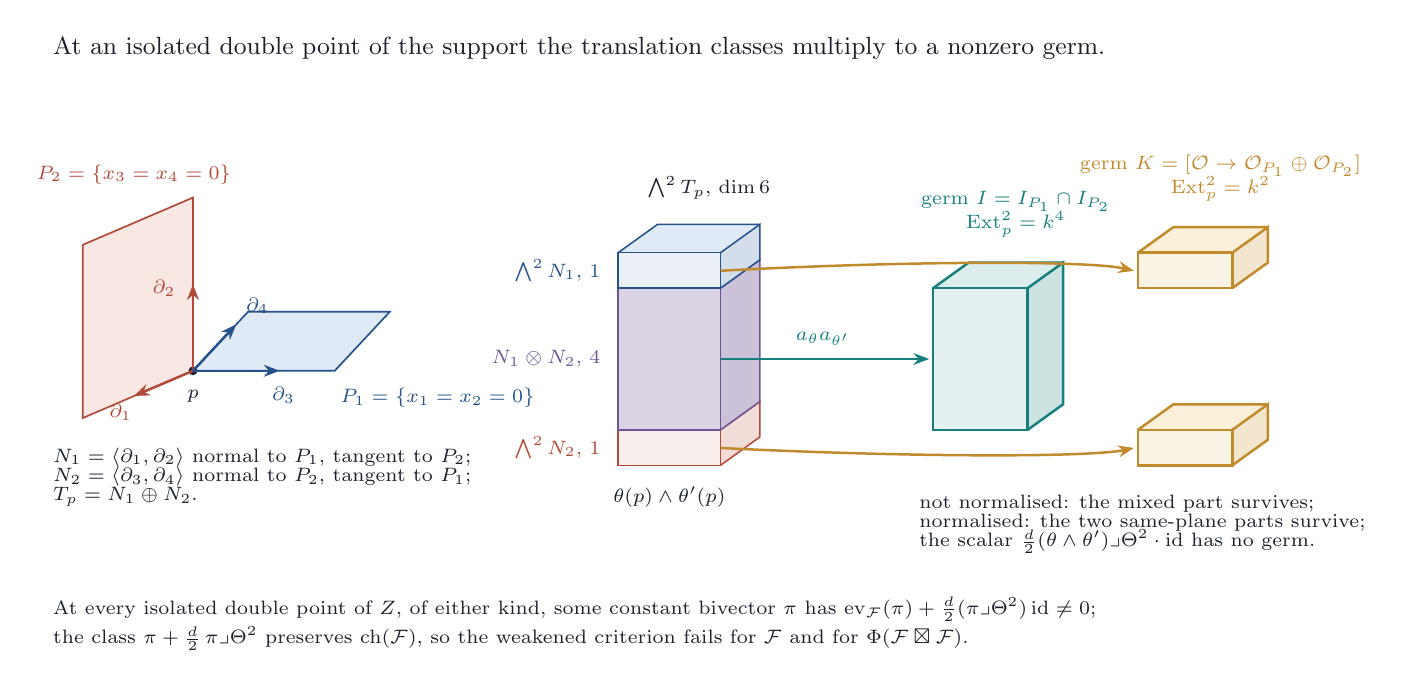
\begin{tikzpicture}[font=\small,text=PInk]

\node[anchor=west,font=\small,text=PInk] at (-0.3,5.3)
  {At an isolated double point of the support the translation classes multiply to a nonzero germ.};

%% =====================================================================
%% Left: the two branches through p
%% =====================================================================
\begin{scope}[shift={(0,0.4)}]
  % P1: a horizontal parallelogram in the (x,y)-plane, corner at p = (1.6,0.8)
  \fill[WBlue,draw=PBlue,line width=0.6pt] (1.6,0.8) -- (3.4,0.8) -- (4.1,1.55) -- (2.3,1.55) -- cycle;
  % P2: a vertical parallelogram, corner at p
  \fill[WClay,draw=PClay,line width=0.6pt,fill opacity=0.92] (1.6,0.8) -- (0.2,0.2) -- (0.2,2.4) -- (1.6,3.0) -- cycle;
  \fill[PInk] (1.6,0.8) circle (1.6pt);
  \node[anchor=north,font=\scriptsize,text=PInk] at (1.6,0.68) {$p$};
  \node[anchor=west,font=\scriptsize,text=PBlue] at (3.35,0.46) {$P_{1}=\{x_{1}=x_{2}=0\}$};
  \node[anchor=south,font=\scriptsize,text=PClay] at (0.85,3.05) {$P_{2}=\{x_{3}=x_{4}=0\}$};
  % normal directions at p: N1 = <d1,d2> is tangent to P2 (drawn along P2), N2 = <d3,d4> tangent to P1
  \draw[PClay,line width=0.9pt,-{Stealth[length=2mm]}] (1.6,0.8) -- (0.85,0.48);
  \draw[PClay,line width=0.9pt,-{Stealth[length=2mm]}] (1.6,0.8) -- (1.6,1.9);
  \node[anchor=north east,font=\scriptsize,text=PClay] at (0.95,0.5) {$\partial_{1}$};
  \node[anchor=east,font=\scriptsize,text=PClay] at (1.5,1.85) {$\partial_{2}$};
  \draw[PBlue,line width=0.9pt,-{Stealth[length=2mm]}] (1.6,0.8) -- (2.7,0.8);
  \draw[PBlue,line width=0.9pt,-{Stealth[length=2mm]}] (1.6,0.8) -- (2.15,1.39);
  \node[anchor=north,font=\scriptsize,text=PBlue] at (2.75,0.72) {$\partial_{3}$};
  \node[anchor=south west,font=\scriptsize,text=PBlue] at (2.15,1.4) {$\partial_{4}$};
  \node[anchor=north west,align=left,font=\scriptsize,text=PInk] at (-0.3,-0.05)
    {$N_{1}=\langle\partial_{1},\partial_{2}\rangle$ normal to $P_{1}$, tangent to $P_{2}$;\\[-1pt]
     $N_{2}=\langle\partial_{3},\partial_{4}\rangle$ normal to $P_{2}$, tangent to $P_{1}$;\\[-1pt]
     $T_{p}=N_{1}\oplus N_{2}$.};
\end{scope}

%% =====================================================================
%% Centre: the bivectors at p as three slabs, heights 1 : 4 : 1
%% =====================================================================
\begin{scope}[shift={(7.0,0)}]
  \slab{0}{0}{0}{1.3}{1.0}{0.45}{vv}
  \slab{0}{0}{0.45}{1.3}{1.0}{1.8}{pp}
  \slab{0}{0}{2.25}{1.3}{1.0}{0.45}{zz}
  \begin{scope}[obl]
    \coordinate (Bt) at (0.65,1.0,2.7);
    \coordinate (Bb) at (0.65,0,0);
    \coordinate (Rlo) at (1.3,0.0,0.22);
    \coordinate (Rmid) at (1.3,0.0,1.35);
    \coordinate (Rhi) at (1.3,0.0,2.47);
    \coordinate (Llo) at (0,0.0,0.22);
    \coordinate (Lmid) at (0,0.0,1.35);
    \coordinate (Lhi) at (0,0.0,2.47);
  \end{scope}
  \node[anchor=south,align=center,font=\scriptsize,text=PInk] at ([yshift=2mm]Bt)
    {$\bigwedge^{2}T_{p}$, $\dim 6$};
  \node[anchor=east,font=\scriptsize,text=PBlue] at ([xshift=-1mm]Lhi) {$\bigwedge^{2}N_{1}$, $1$};
  \node[anchor=east,font=\scriptsize,text=PViolet] at ([xshift=-1mm]Lmid) {$N_{1}\otimes N_{2}$, $4$};
  \node[anchor=east,font=\scriptsize,text=PClay] at ([xshift=-1mm]Llo) {$\bigwedge^{2}N_{2}$, $1$};
  \node[anchor=north,align=center,font=\scriptsize,text=PInk] at ([yshift=-1.5mm]Bb)
    {$\theta(p)\wedge\theta'(p)$};
\end{scope}

%% =====================================================================
%% Right: the two germs and their local Ext^2
%% =====================================================================
\begin{scope}[shift={(11.0,0)}]
  % germ I: Ext^2 = k^4, fed by the middle block
  \slab{0}{0}{0.45}{1.2}{0.9}{1.8}{ker}
  \begin{scope}[obl]
    \coordinate (It) at (0.6,0.9,2.25);
    \coordinate (Il) at (0,0,1.35);
  \end{scope}
  \node[anchor=south,align=center,font=\scriptsize,text=PTeal] at ([yshift=2mm]It)
    {germ $I=I_{P_{1}}\cap I_{P_{2}}$\\[-1pt]$\operatorname{Ext}^{2}_{p}=k^{4}$};
  % germ K: Ext^2 = k^2, fed by the two outer blocks
  \begin{scope}[shift={(2.6,0)}]
    \slab{0}{0}{0}{1.2}{0.9}{0.45}{sig}
    \slab{0}{0}{2.25}{1.2}{0.9}{0.45}{sig}
    \begin{scope}[obl]
      \coordinate (Kt) at (0.6,0.9,2.7);
      \coordinate (Klo) at (0,0,0.22);
      \coordinate (Khi) at (0,0,2.47);
    \end{scope}
    \node[anchor=south,align=center,font=\scriptsize,text=POchre] at ([yshift=2mm]Kt)
      {germ $K=[\mathcal O\to\mathcal O_{P_{1}}\oplus\mathcal O_{P_{2}}]$\\[-1pt]$\operatorname{Ext}^{2}_{p}=k^{2}$};
  \end{scope}
\end{scope}
% arrows: the product map on the bivectors
\draw[PTeal,line width=0.9pt,-{Stealth[length=2mm]}] (Rmid) -- (10.95,1.35);
\draw[POchre,line width=0.9pt,-{Stealth[length=2mm]}] (Rlo) .. controls (10.7,0.1) and (13.0,0.1) .. (13.55,0.22);
\draw[POchre,line width=0.9pt,-{Stealth[length=2mm]}] (Rhi) .. controls (10.7,2.6) and (13.0,2.6) .. (13.55,2.47);
\node[anchor=south,font=\scriptsize,text=PTeal] at (9.6,1.4) {$a_{\theta}a_{\theta'}$};
\node[anchor=north west,align=left,font=\scriptsize,text=PInk] at (10.7,-0.25)
  {not normalised: the mixed part survives;\\[-1pt]
   normalised: the two same-plane parts survive;\\[-1pt]
   the scalar $\tfrac d2(\theta\wedge\theta')\lrcorner\Theta^{2}\cdot\mathrm{id}$ has no germ.};

%% summary line
\node[anchor=north west,align=left,font=\scriptsize,text=PInk] at (-0.3,-1.55)
  {At every isolated double point of $Z$, of either kind, some constant bivector $\pi$ has
   $\operatorname{ev}_{\mathcal F}(\pi)+\tfrac d2(\pi\lrcorner\Theta^{2})\,\mathrm{id}\ne0$;\\[1pt]
   the class $\pi+\tfrac d2\,\pi\lrcorner\Theta^{2}$ preserves $\operatorname{ch}(\mathcal F)$, so the weakened criterion fails for $\mathcal F$ and for $\Phi(\mathcal F\boxtimes\mathcal F)$.};

\end{tikzpicture}
\end{document}
